
\chapter{Erstellung studentischer wissenschaftlicher Arbeiten mit der \emph{KITreprt}-Klasse} % (fold)
\label{cha:erstellung_studentischer_wissenschaftlicher_arbeiten_mit_der_kitreprt_klasse}
Die \emph{KITreprt}-Klasse dient vorrangig der Erstellung studentischer wissenschaftlicher Texte wie zum Beispiel Bachelor- oder Masterarbeiten. 
Aufbauend auf dem \emph{Koma-Script}\footnote{\url{http://www.komascript.de/}} bietet diese Klasse eine KIT-konforme Titelseite, bindet die empfohlenen Pakete
standardmässig ein und versucht ein möglichst ansprechendes Seitenlayout zu erzeugen. In diesem Kapitel werden die Aspekte dieser Klasse
vorgestellt und ein paar generelle Hinweise zur Verwendung von {\LaTeX} aufgezeigt. Dieses Dokument wurde mit dieser Klasse erstellt und 
der Quelltext soll als weiterführendes Beispiel  dienen.

\section{Die \emph{KITreprt}-Klasse}
\subsection{Verwendung der Klasse}
Die Klasse wird mit dem Befehl \lstinline[language={[LaTeX]TeX}]!\documentclass[english,ngerman]{KITreprt}! eingebunden. Die Sprache kann mit dem 
Befehlen \lstinline[language={[LaTeX]TeX},morekeywords={selectlanguage}]!\selectlanguage{ngerman}! und \lstinline[language={[LaTeX]TeX},morekeywords={selectlanguage}]!\selectlanguage{english}! zwischen dem Deutschen und dem Englischen umgeschalten werden. Dokumente mit der \emph{KITreprt}-Klasse sollten direkt mit \emph{Pdflatex} in Pdf-Dokumente übersetzt werden und unbedingt 
\emph{UTF-8} als Zeichenkodierung verwenden.


\subsection{Die Einrichtung der Titelseite}
Das Layout der Titelseite ist komplett in der Klassendefinition enthalten und es werden keine weiteren Dateien, zum Beispiel für das Logo, benötigt.
Für die Daten auf der Titelseite müssen \TeX-Makros definiert (bzw. neu definiert werden). Sind diese nicht gesetzt erscheinen auf der Titelseite 
in roter Schrift Anweisungen, wie diese gesetzt werden müssen. Um ein Makro neu zu definieren reicht zum Beispiel die Anweisung \lstinline[language={[LaTeX]TeX}]!\renewcommand{\myshorttitle}{Die offizielle HIS-\LaTeX-Vorlage}!. Die möglichen Makros sind in Tabelle~\ref{tab:makros} aufgelistet. Eine Ausnahme bilden
die Makros \texttt{\textbackslash  advisor}, \texttt{\textbackslash  advisortwo}, \texttt{\textbackslash  reviewer} und \texttt{\textbackslash  reviewertwo}. 
Dies müssen mit \texttt{\textbackslash  newcommand} komplett neu definiert werden, um auf der Titelseite zu erscheinen. Ist keins dieser vier Makros
definiert, muss ein spezielles Makro definiert werden, damit kein roter Text zu sehen ist:  \lstinline[language={[LaTeX]TeX}]!\renewcommand{\noadvisors}{}!.
\begin{table}[h]
\centering
\begin{tabular}{cl}
\toprule
Makro & Inhalt \\
\midrule 
\texttt{\textbackslash myname} & \emph{Name des Autors} \\
\texttt{\textbackslash mythesis} & \emph{Vordefiniert (zweisprachig):} \texttt{\textbackslash termpaper} \emph{(Seminararbeit)}, \texttt{\textbackslash mastersthesis}, \\
&  \texttt{\textbackslash bachelorsthesis}, \texttt{\textbackslash protocol},  \texttt{\textbackslash studienarbeit}, \\
& \texttt{\textbackslash diplomarbeit}, \emph{oder eigene Bezeichnung} \\
\texttt{\textbackslash myshorttitle} & \emph{Name der Arbeit} \\
\texttt{\textbackslash mytitle} & \emph{Optionaler Untertitel oder leer } \\
\texttt{\textbackslash timestart} & \emph{Anfangsdatum} \\
\texttt{\textbackslash timestart} & \emph{Datum der Abgabe} \\
\texttt{\textbackslash  advisor} & \emph{Name des betreuenden Mitarbeiteiters (Seminararbeiten)} \\
\texttt{\textbackslash  reviewer} & \emph{Name des Referenten} \\
\bottomrule
\end{tabular}
\caption{Die Makros die für die Titelseite definiert werden müssen. Tabellen in wissenschaftlichen Texten sollten nach Möglichkeit nie 
vertikale Linien verwenden. }
\label{tab:makros}
\end{table}

\subsection{Vordefinierte Pakete }
Die folgenden Pakete werden in der \emph{KITreprt}-Klasse definiert und müssen daher nicht von Hand eingebunden werden.
\begin{description}
\item[\emph{babel}] Lokalisierte Trennung und Schriftsatz. 
\item[\emph{fontenc}] Umlaute und Sonderzeichen.
\item[\emph{inputenc}] \emph{Utf-8} Zeichenkodierung. Dokumente müssen diese Kodierung verwenden, um mit der Klasse verwendet werden zu können.
\item[\emph{graphicx}] Für die Einbindung von Graphiken in moderenen Formaten.
\item[\emph{amsmath,amssymb,amsthm,bm,bbm}] Mathematische Symbole und Extrapakete.
\item[\emph{color}] Für farbigen Text. Die Farbe \gqq{grey} wird auch in der Klasse definiert.
\item[\emph{subfigure}] Mehrere Einzelbilder in der selben Abbildung.
\item[\emph{booktabs}] Ansprechende Tabellen (siehe~Tab.~\ref{tab:makros}).
\item[\emph{listings}] Darstellung von Quelltexten (siehe Abschnitt~\ref{sec:code}).
\item[\emph{helvet,courier,mathptmx}] Alternative Schriften (z.B. Serifenlose Schrift für Überschriften.
\item[\emph{lastpage}] Erlaubt die letzte Seite zu referenzieren
\item[\emph{natbib}] Paket zum Zitieren für die Naturwissenschaften. Der Stil \emph{abbrvnat} ist voreingestellt.
\item[\emph{tikz,eso-pic,setspace,automark}] Pakete, die intern zum Beispiel für die Titelseite verwendet werden.
\end{description}

\subsection{\LaTeX-Befehle}

Dieses Dokument soll nicht als ausführliche Einführung in \LaTeX{} verstanden werden. Für eine Übersicht über alle
Befehle, wie zum Beispiel\lstinline[language={[LaTeX]TeX}]!\emph! für hervorgehobenen Text, wird daher auf folgende Quellen verwiesen:
\begin{itemize}
\item Die deutsche \href{http://de.wikipedia.org/wiki/LaTeX}{Wikipedia-Seite zu \LaTeX}\footnote{http://de.wikipedia.org/wiki/LaTeX} verweist auf einige gute Einführungen.
\item Der \LaTeX Companion von \citet*{latexcompanion}.
\end{itemize}



\section{Verweise und Zitate}
\subsection{Verweise}
\label{sec:ref}
Um auf Stellen im selben Dokument zu verweisen wird der \lstinline[language={[LaTeX]TeX}]!\ref!-Befehl verwendet. Dazu müssen 
an den Betreffenden Stellen Markierungen (sogenannte Labels) mit dem\lstinline[language={[LaTeX]TeX}]!\label!-Befehl gesetzt werden.
Üblicherweise werden so Textstellen wie Kapitel und Abschnitte oder Abbildungen und Tabellen markiert. Bei 
Textstellen können direkt nach dem entsprechenden Befehl die Markierungen gesetzt werden, bei Abbildungen sowie Tabellen 
muss dies nach dem Festlegen der Überschrift passieren. 
Die Verweise können von \LaTeX erst nach wiederholtem Übersetzen korrekt aufgelöst werden.
Es empfiehlt sich die Markierungsbezeichnungen zu strukturieren, zum Beispiel alle Abbildungen mit einem vorausgehenden \emph{fig:} 
zu kennzeichnen.
\subsection{Zitate}
Für das Zitieren soll unbedingt \emph{Bibtex}\footnote{Weitere Informationen unter \url{http://www.bibtex.org/de/}} verwendet werden.
Das \emph{natbib}-Paket\footnote{\url{http://www.ctan.org/pkg/natbib}} stellt zusätzliche Befehle zum Zitieren zur verfügung:
\begin{description}
\item[\texttt{citet}] Dieser Befehl erzeugt Zitate, die direkt im Text erscheinen: \citet{Asfour2006}, 
\item[\texttt{citet}$\ast$] Das Asterisk lässt alle Koautoren erscheinen: \citet*{Asfour2006}
\item[\texttt{citep}] Mit diesem Befehl werden Zitate in Klammern angezeigt: \citep{Asfour2006}
\end{description}
\emph{Wichtig:} Nicht nur direkte Zitate, die in Anführungszeichen (im Deutschen der Befehl \lstinline[language={[LaTeX]TeX}]!\gqq!) gekennzeichnet werden müssen, sondern auch alle Gedanken, Ideen oder Ansätze,
die nicht vom Autor stammen müssen korrekt und vollständig zitiert werden.
\subsection{Zeilenumbrüche}
Die \emph{cite}- und \emph{ref}-Befehle sollten immer durch eine vorangestellte Tilde ($\sim$) -- das steht in \LaTeX{} ein geschütztes Leerzeichen -- direkt mit vorhergehenden Wort verbunden werden, damit kein unerwünschter
Zeilen- oder Seitenumbruch dazwischen erfolgen kann.\\Zum Beispiel: \lstinline[language={[LaTeX]TeX},morekeywords={citep}]! Der Roboter Armar-III~\citep{Asfour2006} hat sieben Freiheitsgrade pro Arm.!

\section{Bilder und Tabellen}
In \LaTeX sollten Bilder und Tabellen prinzipiell nicht an einer festen Stelle an den Text gekoppelt werden. Vielmehr gibt es dafür Umgebungen (sogenannte 
\emph{floating}-Umgebungen), die die Bilder automatisch in der Nähe und an typographisch sinnvoller Stelle platzieren. 
Für Abbildungen steht dafür die \emph{figure-} und für Tabellen die \emph{tabular-}Umgebung zur Verfügung. 
\subsection{Bilder}
Die Verwendung der \emph{figure}-Umgebung soll hier anhand eines kurzen Beispiels in Listing~\ref{lst:float} erläutert werden. Die 
resultierende Abbildung ist Abb.~\ref{fig:example}.

\begin{center}
\begin{minipage}{0.65\textwidth} 
\begin{lstlisting}[language={[LaTeX]TeX},caption={Beispiel für eine Floatumgebung.},morekeywords={subfigure,includegraphics},label={lst:float}]
\begin{figure}[htbp]
\begin{center}
% Die beiden Teilbilder
\subfigure[Die humanoiden Roboter ARMAR-IIIa und ARMAR-IIIb am His.]{
\label{fig:example2a}
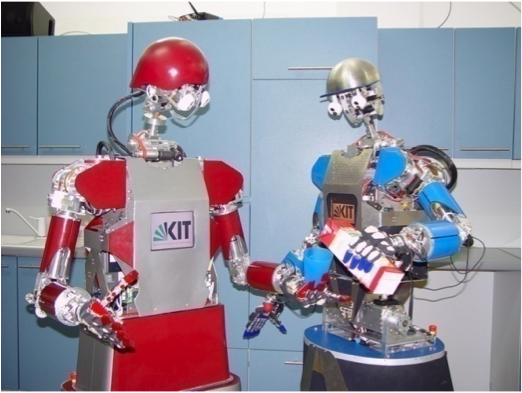
\includegraphics[width=0.3\textwidth]{Example1}}    
% horizontaler Abstand  von 1cm.
\hspace{1cm}            
\subfigure[Der Kopf des Roboters ARMAR-IIIa]{
\label{fig:example2b}
\includegraphics[width=0.3\textwidth]{Example2}}                
% Ueberschrift und Verweismarke fuer die gesamte Abbildung.
\caption{Die Roboter des HIS.}
\label{fig:example}
\end{center}
\end{figure}
\end{lstlisting}
\end{minipage}
\end{center}

\begin{figure}[htbp]
\begin{center}
\subfigure[Die humanoiden Roboter ARMAR-IIIa und ARMAR-IIIb am His.]{\label{fig:example2a}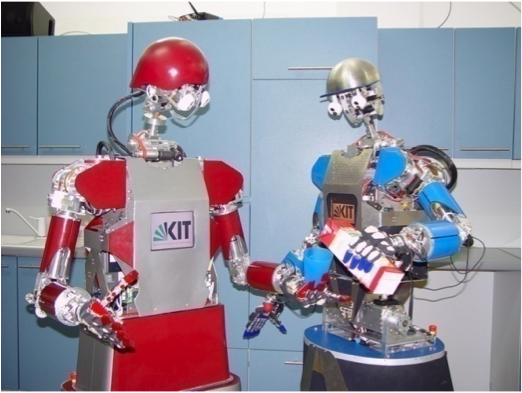
\includegraphics[width=0.3\textwidth]{Example1}}    
\hspace{1cm}            
\subfigure[Der Kopf des Roboters ARMAR-IIIa]{\label{fig:example2b}\includegraphics[width=0.3\textwidth]{Example2}}                
\caption{Die Roboter des HIS.}
\label{fig:example}
\end{center}
\end{figure}


Die eckigen Klammern umfassen die optionalen Parameter, die die Platzierung der Abbildung (nicht zwingend) beeinflussen. 
Die Parameter sind Präferenzen und \LaTeX{} versucht sie der Reihe nach zu erfüllen:
\begin{description}
\item[h] Direkt an der Stelle, wo es definiert wurde.
\item[t] Oben, am Anfang der Seite.
\item[b] Unten, am Ende der Seite.
\item[p] Gesondert, auf einer Extraseite für Abbildungen.
\end{description}
In der Umgebung ist eine \emph{center}-Umgebung eingeschlossen, die das Bild zentriert erscheinen lässt. 
Die beiden \emph{subfigure}-Befehle erzeugen die Einzelbilder der Abbildung. Die optionalen Parameter in eckigen Klammern
erzeugen die Bildunterschriften der Einzelbilder. Gefolgt in den geschweiften Klammern können Markierungen für Verweise auf die Einzelbilder angelegt werden (z.B. für Abb.~\ref{fig:example2a})
und mittels \texttt{\textbackslash includegraphics} wirklich die Graphikdatei in das Dokument eingebunden werden. 
Wenn das Bild im Suchpfad liegt (siehe unten) ist keine vorangehende
Pfadangabe und Dateierweiterung nötig. 
Der \emph{caption}-Befehl weiter unten erlaubt eine Überschrift für die gesamte Abbildung anzugeben. Die Markierung mittels
\emph{label} wird in Abschnitt~\ref{sec:ref} behandelt. Die geöffneten Umgebungen müssen mit einem \emph{end} wieder geschlossen 
werden. Anstelle der \emph{subfigure}-Befehle kann auch ein einzelnes \emph{includegraphics} stehen.
Der Graphikpfad kann wie folgt gesetzt werden (man beachte die doppelten geschweiften Klammern und dass die Anweisung vor dem
Dokumentanfang stehen muss):\\
\lstinline[language={[LaTeX]TeX}]!\graphicspath{{./images/}}!


\subsection{Tabellen}
Die Umgebung für Tabellen ähnelt stark derer für Bilder -- inklusive Überschriften und Textmarken. Leider sind die Tabellen selbst 
relativ kompliziert in \LaTeX. Daher wird an dieser Stelle auf den Quelltext dieses Dokuments und 
andere Quellen verwiesen\footnote{\url{http://en.wikibooks.org/wiki/LaTeX/Tables}}.
In Tabellen sollten generell vertikale Linien vermieden werden, um ein modernes Erscheinungsbild zu garantieren. Das \emph{booktabs}-Paket\footnote{\url{http://ctan.org/tex-archive/macros/latex/contrib/booktabs/}} ermöglicht hier die Verwendung unterschiedlich dicker Linien mit \texttt{\textbackslash toprule},
\texttt{\textbackslash midrule} und \texttt{\textbackslash bottomrule} (siehe Tab.~\ref{tab:makros}). 


\section{Quelltexte}\label{sec:code}
Um Quelltexte (engl. Listings) wie in Listing~\ref{lst:float} zu setzen sollte das \emph{listings}-paket\footnote{\url{http://www.ctan.org/tex-archive/macros/latex/contrib/listings/}} verwendet werden. Listings in \emph{float}-Umgebungen
werden mit abgerundeten Rahmen gemäss der Titelseite versehen und unterstützen Syntaxhighliting (farbliche Kennzeichnung von Spracheigenheiten). Als Standard-Sprache ist nach einbinden der Klasse \emph{C++} voreingestellt.

 So kann man
zum Beispiel mit \lstinline[language={[LaTeX]TeX}]-\lstinline[language={[LaTeX]TeX}]!\emph!- \LaTeX-Befehle im Text eingebettet anzeigen. Für weitere Beispiele sollte der Quelltext dieses Dokuments untersucht werden.
% chapter erstellung_studentischer_wissenschaftlicher_arbeiten_mit_der_kitreprt_klasse (end)
